%%=============================================================================
%% Uitwerking
%%=============================================================================

\chapter{Uitwerking}
\label{ch:uitwerking}


\section{Benodigdheden}
\label{sec:Benodigdheden}

\subsection{Data}
Een onmisbaar onderdeel om aan machine learning te doen is uiteraard de data. Tijdens de eerste fases van het project wordt er gebruik gemaakt van zelf gegenereerde data in Excel. De data die uit de arcademachine ontvangen zal worden zal in CSV-formaat zijn. Doordat Excel-tabbladen opgeslagen kunnen worden in een CSV-file is dit dan ook een logische keuze. 
Er zullen zo'n 500 metingen beschikbaar zijn die kunnen ingelezen worden in het programma. 

We willen uiteraard weten hoe goed het algoritme scoort dit kunnen we testen door testdata te voorzien. De dataset die we uit Excel halen zal opgesplitst worden in trainingsdata en testdata. Het algoritme zal met de trainingsdata een hypothese vormen die ervoor zal zorgen dat ook nieuwe of nog ongekende data een goede voorspelling krijgt. Daarom is het belangrijk om een dataset te hebben die data bevat die nog niet eerder gebruikt is door het algoritme. Enkel op deze manier kunnen we zeker zijn dat het algoritme een goede hypothese heeft gemaakt. Als testdata nemen we 20\% van de hele dataset. 

\subsection{Frameworks}
Zoals in de inleiding reeds besproken was zijn er verschillende soorten frameworks die reeds geïmplementeerde algoritmen hebben. Een eerste mogelijk framework was TensorFlow van Google. Dit is ontwikkeld in Python, de algoritmen die hierin voorzien zijn, zijn voornamelijk neurale netwerken of deep learning algoritmen. Het is mogelijk om ook eenvoudigere algoritmen te gebruiken maar daar ligt de specialiteit niet op. En dit in combinatie met een taal die ik niet machtig ben lijkt mij geen goede keuze. Er zijn nog een aantal andere frameworks die gemaakt zijn in andere programmeertalen zoals Javascript, Node.js, Java, etc. 

Accord-framework is daar een van, dit is ontwikkeld in .NET. Alle algoritmen die nodig zijn om deze bachelorproef tot een succesvol einde te brengen zijn beschikbaar. \newline
Door te werken met het Accord-framework bestaat er een mogelijk om in de toekomst een webapplicatie te ontwikkelen. Dit openend dus ook nog extra mogelijkheden om te experimenteren met Artificiële Intelligentie. 
\newline
.NET is een nog niet zo'n populaire taal om aan artificiële intelligentie te doen maar er zit potentieel in. Doordat .NET vele gelijkenissen heeft met Java is er een nog groter publiek die hiermee aan de slag kan.
\newline
Door deze mogelijkheden lijkt dit dan ook het meest geschikte framework om aan het werk te gaan. 

\section{Fase 1}
\label{sec:Fase1}
De eerste stap om een programma te maken om voorspellingen te doen is de data maken. Omdat dit ook nog maar de eerste fase is beginnen we gemakkelijk. Dit wil zeggen dat we de computer een eerste voorspelling laten doen tussen twee totaal verschillende spelletjes. We nemen Pacman en Mortal Kombat (schietspel) om te starten. Pacman kan gespeeld worden enkel d.m.v. joystickbewegingen. Om Mortal Kombat te spelen heb je veel de knoppen nodig maar ook de joystick.  Nu als mens is het gemakkelijk om dit verschil te kunnen zien, als er knoppen gebruikt geweest zijn kunnen we concluderen dat de speler Mortal Kombat aan het spelen was. 

\subsection{Data}
\label{sec:DataFase1}
De eerste dataset is zelf gegenereerd zonder echte input van de arcademachine omdat het systeem die de data zal inlezen nog in ontwikkeling is op dit moment. 
In Excel zijn er drie kolommen voorzien een kolom voor het aantal keer dat de knoppen ingedrukt zijn geweest gedurende twee minuten. Dan het aantal keer dat de joystick bewogen is in diezelfde tijdsspanne. De derde kolom staat het ID van het spel. 
In figuur \ref{fig:regressieFig} op pagina \pageref{fig:regressieFig} ziet u random 10 voorbeelden uit de dataset.
Het GameID 0 wijst op Pacman en 1 is dan Mortal Kombat. Als u de rijen van Pacman bekijkt dan valt op dat de ButtonPresses niet 0 zijn, dit komt omdat er bij het begin van een spel soms eens geprobeerd wordt wat de functies van de knoppen zijn. 

\begin{figure}[]
	\centering
	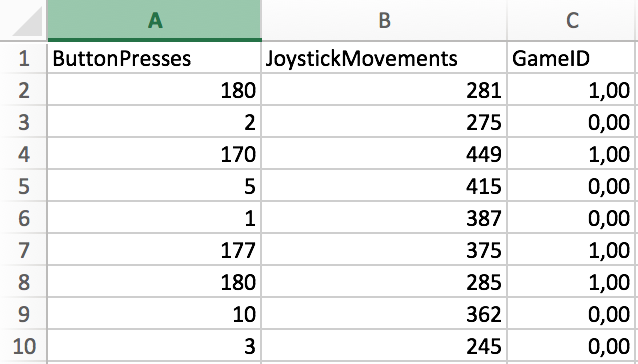
\includegraphics{img/Dataset}
	\caption{Tien voorbeelden van games}
	\label{fig:regressieFig}
\end{figure}


\newpage

\subsection{Logistische regressie}
\label{sec:Logistischeregressie-fase1}

Het eerste algoritme die we gaan testen is logistische regressie. In fase 1 gaan we slecht voorspellingen doen tussen twee verschillende spellen vandaar dat we binaire logistische regressie gaan toepassen die eerder uitgelegd is in sectie \ref{sec:Binaire-logistische-regressie}.

In de code \ref{code:linaireRegressieTweeKlassen} ziet u de implementatie van de binaire logistische regressie. Er worden twee parameter meegegeven in de functie, input en output. De input is een dubbele array van \textit{double} waarden. Daarin zitten rijen met twee kolommen die de ButtonPresses en JoystickMovements bevatten. De ouput parameter bevat een enkele array die het GameID bevat. Hoe deze data ingelezen wordt kan u zien in de code \ref{code:dataInlezen} op pagina \pageref{code:dataInlezen}. Met een ExcelReader krijgen we een DataTable die we met de methode ToJagged kunnen omvormen naar ons gewenste dubbele array met de kolomnamen kunnen we de kolommen selecteren. Deze methode is onderdeel van het Accord-framework. 


%\textit{Wat de LearningRate precies inhoudt wordt later samen met gradient descent uitgelegd (gradient descent zal in het theoretische deel uitgelegd worden)}

\subsubsection{Resultaten}
\paragraph{Snelheid van het algoritme} 
Een eerste belangrijke metric om algortimen te kunnen vergelijken is de snelheid. Het zou niet correct zijn om een stopwatch te laten lopen bij het begin van het programma en te stoppen wanneer het programma klaar is. De tijd om de data in te laden in het programma, de omzetting naar arrays, de objecten die worden geïnitialiseerd, ... is allemaal niet zo belangrijk. Wat wel interessant is, is de tijd die het algoritme nodig heeft om tot een hypothese te komen. Dit gebeurt in de \textit{Learn} methode. 
Net voor die lijn code wordt uitgevoerd starten we een stopwatch en erna stoppen we en bekijken het verschil. Omdat de duur verschillend kan zijn nemen we het gemiddelde van 50 metingen. 
Doordat deze dataset slechts 400 voorbeelden bevat en de verschillen tussen de spelletjes Pacman en Mortal Kombat zeer duidelijk zijn heeft het algoritme slechts 5,8302 milliseconden nodig om een hypothese te maken. Dit resultaat is het gemiddelde van twintig testen. 
\paragraph{F-score} 

Doordat deze dataset zo simpel is en de testdataset dus ook heeft het algoritme geen probleem om de testdata te classificeren. De precisie is dan ook logischerwijs één en de rappel eveneens.
Zo bekomen we een precisie van 1 die dus wil zeggen dat het algoritme foutloos is op de testdata.  


\textit{Als ik meer data zou voorhanden hebben kan ik de McNeymar's test doen maar in deze fase en deze hoeveelheid data is die test niet echt handig}

%%Logistic regression code
\begin{figure}[]
	\renewcommand{\figurename}{Code}
\begin{lstlisting}
public static void StartLogisticRegression(double[][] input, int[] output)
{
       //LogisticRegression object initialiseren met 2 inputparameters (ButtonPresses & JoystickMovements)
       LogisticRegression logisticRegression = new LogisticRegression()
       {
       		NumberOfInputs = 2
       };
       
      var learner = new LogisticGradientDescent(logisticRegression)
       {
            Tolerance=0.1
       };
    
     // De gradient descent begint met de logistische regressie te optimaliseren
     logisticRegression = learner.Learn(input, output);
}

\end{lstlisting}
\caption{Implementatie binaire logistische regressie}
\label{code:linaireRegressieTweeKlassen}
\end{figure}
%%Data inlezen
\begin{figure}[]
	\renewcommand{\figurename}{Code}
	\begin{lstlisting}
using (var table = new ExcelReader("../../datasetExcel.xls").GetWorksheet("Training"))
   {
       // Convert the DataTable to input and output vectors
       double[][] inputs = table.ToJagged<double>("ButtonPresses", "Joystickmovements");
       int[] outputs = table.Columns["Game"].ToArray<int>();
       
       ...
   }
	\end{lstlisting}
	\caption{Inlezen Excel data}
	\label{code:dataInlezen}
\end{figure}

\newpage
\subsection{Support Vector Machine}
\label{sec:supportvectormachine}
Support Vector Machine is het tweede algoritme die we zullen gebruiken en dus vergelijken met logistische regressie. 
We zijn nog altijd in de eerste fase dus vergelijken we twee klassen met elkaar. 
De code voor Support Vector Machine vindt u in code \ref{code:svmBi} op pagina \pageref{code:svmBi}. 

De parameters inputs en outputs worden opnieuw meegegeven nadat de data is opgehaald zoals we gezien hebben in code \ref{code:dataInlezen}. Vervolgens initialiseren we het SupportVectorMachine object. We geven in de constructor het aantal features mee (in het Accord-framework gebruiken ze inputs wat verwarrend kan zijn). Het aantal features in dit geval is 2 namelijk de kolommen ButtonPresses en Joystickmovements. Vervolgens wordt het optimalisatie algoritme gecreëerd met de nodige attributen die voor zichzelf spreken. Tot slot kan de SVM geoptimaliseerd worden d.m.v de Learn methode.  

\subsubsection{Resultaten}
\paragraph{Snelheid van het algoritme} 
Om de snelheid van dit algoritme te meten plaatsen we opnieuw een stopwatch voor net voor het de lijn \textit{"svm = teacher.Learn(inputs, outputs)"}. En we stoppen die uiteraard net nadat deze lijn is uitgevoerd. Het programma is 20 keer uitgevoerd geweest en daarvan is het gemiddelde genomen van de 20 resultaten. 30,4823 milliseconden is hoelang Support Vector Machine nodig heeft om een hypothese te stellen. En dit met een standaard deviatie van slechts 1,3146.

\paragraph{F-score}
Doordat deze dataset zo simpel is net zoals de testdataset, heeft het algoritme geen probleem om de testdata te classificeren. De precisie is dan ook logischerwijs één net als de rappel.
Zo bekomen we een precisie van 1 die dus wil zeggen dat het algoritme foutloos is op de testdata.  



%%svm 2-class
\begin{figure}[]
\renewcommand{\figurename}{Code}
\begin{lstlisting}
public static void StartSupportVectorMachine(double[][] inputs, int[] outputs)
{
//Support Vector Machine initialiseren met 2 input features namelijk ButtonPresses en Joystickmovements
SupportVectorMachine svm = new 			SupportVectorMachine(inputs: 2);
	//Het optimalisatiealgoritme voor SVM van het Accordframework is als vlogt geinitialiseerd
	var teacher = new LinearDualCoordinateDescent()
	{
	      Inputs = inputs,
	      Outputs = outputs,
	      Model = svm,
	      Tolerance = 0.1
	};
	//SVM wordt geoptimaliseerd
	svm = teacher.Learn(inputs, outputs);
}
\end{lstlisting}
\caption{Support Vector Machine implementatie}
\label{code:svmBi}
\end{figure}
\subsection{Conclusie na fase 1}
Bij een eerste vergelijking met twee inputvariabelen en twee klassen. Aangezien dit een simpele start is met twee duidelijk verschillende spelletjes hebben beide algoritmen een perfecte F-score van 1.  Het verschil wordt nu dus gemaakt op de snelheid. Logistische regressie had een hypothese geleerd in 5,8302 milliseconden terwijl de SVM daar gemiddeld 30,4823 over gedaan heeft. Dit $\pm$ 5 keer langer. 
\newline
Op dit ogenblik krijgt logistische regressie logischerwijs nog de voorkeur. Uiteraard zal in de arcade machine meerdere spelletjes beschikbaar zijn. Ook zullen er meer dan twee metrics zijn waarop we spelletjes kunnen vergelijken. 



\newpage
\section{Fase 2}
\label{sec:Fase2}

In \ref{sec:Fase1} fase 1 maakten we gebruik van ButtonPresses en JoystickMovements. We gaan nu nog een extra inputvariabele toevoegen. Er zijn spelletjes waar je soms eventjes niet kan spelen omdat er van level wordt veranderd of als je bijvoorbeeld Pacman speelt wordt er afgeteld van 3 naar 1 wanneer je dood geweest bent, dit zijn dan 3 seconden dat er niets gebeurt is. Terwijl er bij Mortal Kombat meer gespeeld wordt en minder lang moet wachten.
Vandaar dat er een kolom 'TotalTimeOfNoUseOfControls' is toegevoegd aan de dataset met random getallen die voor Mortal Kombat tussen 800 ms en 2500 ms liggen. Terwijl er bij Pacman gestart wordt vanaf 3000 ms tot 5000 ms.
Doordat er nu een extra variabele toegevoegd is gaan we ervan uit dat de algoritmen er beetje langer over zullen doen dan in de vorige fase. Nadat we deze extra inputvariabele besproken hebben gaan we de dataset nog beetje realistischer te maken. Er zullen nog twee extra inputvariabelen toegevoegd worden namelijk de frequentie van de buttons en joystick per 20 seconden.  

\subsection{Logistische regressie}
\label{sec:Logistischeregressie-fase2}

Omdat we nog altijd met twee klassen werken moet er bijna niets aan de implementatie veranderd worden. Enkel bij de declaratie van het object moet 'NumberOfInputs' naar 3 veranderd worden en vervolgens naar 5 wanneer we de kolommen 'ButtonPressesPer20Seconds' en 'JoystickmovementsPer20Seconds' in het algoritme willen betrekken. 

\subsubsection{Resultaten}
\paragraph{Snelheid van het algoritme} 
We beginnen bij onze eerste extra kolom, 'TotalTimeOfNoUseOfControls'. De snelheid van het algoritme werd opnieuw 20 keer gemeten en met een gemiddelde van 8,6405 ms is wat al  dubbel zo lang is als de eerste implementatie. Dit komt doordat het verschil tussen Pacman en Mortal Kombat nu niet meer afhankelijk is van 2 duidelijk verschillende inputvariabelen maar nu één extra is waar de verschillen dichter bij elkaar liggen.

In de volgende test voegen we de kolommen 'ButtonPressesPer20Seconds' en 'JoystickmovementsPer20Seconds' toe.  Verrassend genoeg is het gemiddelde met deze variabelen erbij slechts .7 ms gestegen. Dit kan verklaard worden doordat er een correlatie is tussen het aantal keer er op een knop gedrukt is in 1 minuut en de frequentie van de knoppen. Om de test te doen hebben we de correlatie tussen die twee kolommen berekent en die komt uit op 0.8010, wat wil zeggen dat er een sterk verband is. Doordat er zo'n sterk verband is brengen die extra inputvariabelen geen meerwaarde aan de dataset. 

Een andere inputvariabele die we kunnen gebruiken is het aantal keer dat de speler 'dood' is geweest. In termen van Pacman is dit iedere keer wanneer hij opgegeten wordt. In geval van Mortal Kombat, het aantal keer de speler dood geschoten is geweest. In beide spelletjes is het mogelijk dat er geen enkele keer een 'dood' is geweest. Of als de speler een beginner is kan die vrij veel 'dood' gegaan zijn. Dit geldt voor beide spelletjes.  Wanneer we de gemiddelden meten van met deze kolom erbij dan krijgen we een gemiddelde van 8 ms. De verklaring waarom het algoritme niet veel meer vertraagt is omdat de waarden van de eerste twee kolommen veel zwaarder doorwegen dan de laatste twee die nu toegevoegd geweest zijn. Dit geldt ook voor een 5de kolom die toegevoegd zal worden om de moeilijkheid nog beetje te vergroten.  'Multiplayer' is een kolom met boolean waarden. Wanneer er 2 spelers tegen elkaar aan het spelen waren zal die waarde op true staan, anders op false. Pacman zal altijd alleen gespeeld worden dus die waarde zal altijd false zijn.  

Als we het programma debuggen kunnen we de coëfficiënten bekijken. Als we die uitschrijven voor de logistische regressie tot nu toe dan krijgen we volgend functievoorschrift. Daarin ziet u duidelijk dat de laatste 2 kolommen eigenlijk overbodig zijn. 
$$
{y(x0, x1, x2, x3, x4) = 255,958*x0 + 230,2784*x1 + -37,0513*x2 + 0,1878*x3 + 0,7306*x4 + 0,858}
$$
Zoals we in de sectie \ref{sec:Binaire-logistische-regressie} binaire logistische regressie hebben gezien moet de waarde van de functie hierboven nog verwerkt worden in de sigmoïdfunctie. 
 

\paragraph{F-score} 

De logistische regressie met een Tolerance van 0.1 is nog steeds foutloos dus blijft de F-score gelijk aan 1.

%%Logistic regression code
\begin{figure}[]
	\renewcommand{\figurename}{Code}
\begin{lstlisting}
public static void StartLogisticRegression(double[][] input, int[] output)
{
       //LogisticRegression object initialiseren met 5 inputvariabelen
       LogisticRegression logisticRegression = new LogisticRegression()
       {
       		NumberOfInputs = 5
       };
		
		...
}

\end{lstlisting}
\caption{Implementatie binaire logistische regressie met 5 inputvariabelen}
\label{code:linaireRegressieTweeKlassenM5}
\end{figure}


\newpage
\subsection{Support Vector Machine}
\label{sec:supportvectormachineFase2}
Voor de support vector machine gaan we uiteraard dezelfde kolommen gebruiken als dat we voor logistische regressie hebben gedaan. Als het aantal inputvariabelen relatief klein zijn tegenover het aantal trainingsvoorbeelden dan wordt er aangeraden om logistische regressie te gebruiken of een SVM zonder kernel. \autocite{courseraSVM}. Met geen kernel wordt de standaard lineaire kernel bedoelt. Dit is dan ook de kernel die in deze bachelorproef gebruikt wordt.
Ook voor dit algoritme moeten we niet veel aanpassen om meerdere inputvariabele in rekening te brengen. 

\subsubsection{Resultaten}
\paragraph{Snelheid van het algoritme} 
We starten met 'TotalTimeOfNoUseOfControls' toe te voegen. Het algoritme heeft daarvoor gemiddeld 39,3622 ms voor nodig gehad om een hypothese te bekomen. Dit is slechts een vermeerdering van $\pm$ 5 milliseconden. Ook voor de andere twee extra inputvariabelen bedraagt de vermeerdering bijna niets. Dit komt door de Tolerance waarde in het LineaarDualCoordinateDescent object. Die staat standaard ingesteld op 0.1 wat een goede keuze is. Omdat we niet willen dat onze hypothese 'overfit' heeft. Bij SVM's kan de Tolerance waarde niet veranderd worden Overfit is een term die gegeven wordt aan hypothesen die te nauwkeurig zijn wat uiteraard niet goed is. Zo kan het zijn dat nieuwe voorbeelden slecht gegeneraliseerd worden. 


\paragraph{F-score}

Ook de support vector machine is nog altijd feilloos in het voorspellen van de testdata. 


\subsection{Conclusie na fase 2}
Ondanks dat we ondertussen al gebruik maken van vijf inputvariabelen hebben de algoritmen het nog niet moeilijk om correcte voorspellingen te doen. De Tolerance staat voor beiden algoritmen op 0.1 wat aanduidt wanneer een leerproces mag stoppen. Als die waarde de laag staat ingesteld dan zal de hypothese overfitten. Als een hypothese overfitted is dan wil dit zeggen dat hij te nauwkeurig wil voorspellen. Dit kan leiden tot een slechte generalisatie en dus slechte scores op de testdata. Als de Tolerance waarde te hoog is zal de hypothese te algemeen zijn en dus ook niet goed scoren. 





